\chapter{Introducción}

A partir del análisis de sentimiento se generaron hiperparámetros de clasificación, correspondientes a pesos asignados de acuerdo a las palabras negativas o positivas identificadas, así como una composición de adjetivos que reflejen objetividad o subjetividad en las expresiones lingüísticas.\\

Esta información nos es de utilidad ya que podemos conocer el sentimiento de respuesta general del publico en sus comentarios, ver el tipo de reacción que tiene sobre el publico, e incluso podría permitir la clasificación del publico objetivo, así como temas de discusión o o identificar comportamiento negativo.\\

\chapter{Descripción de los datos}

Para este reporte se emplean los comentarios en vivo, aportados por usuarios de YouTube durante el primer debate presidencial de México 2024, tal como lo observamos en los reportes anteriores.\\

\begin{figure}[!h]
	\centering
	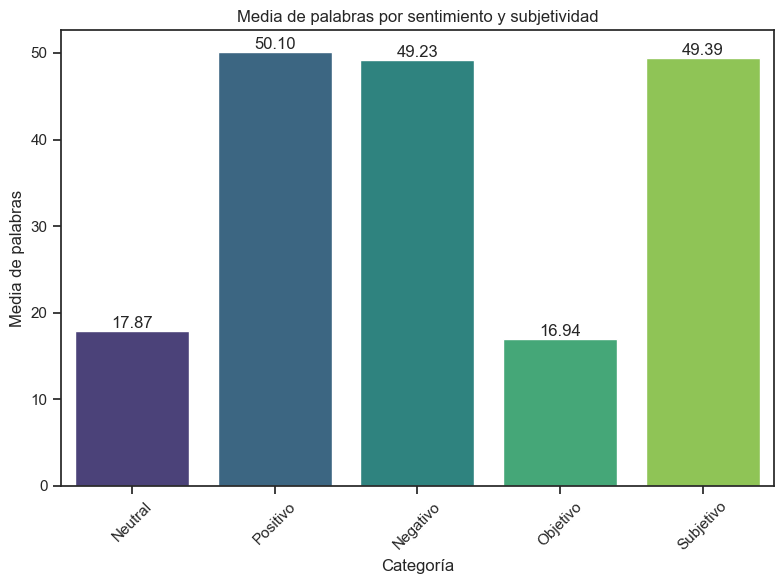
\includegraphics[width=14cm]{Images/Promedio_de_palabras}
	\caption{Distribución de promedio de palabras por sentimiento y objetividad.}
	\label{fig:promediodepalabras}
\end{figure}

Del conjunto de datos, al procesar y clasificar las respuestas del análisis de sentimiento y subjetividad, se realiza la clasificación de los comentarios con base en el valor obtenido de cada escala para cada parámetro, por lo que podemos clasificar los comentarios en 5 tipos distintos; clasificando los comentarios con sentimiento: positivo, neutral y negativo; 2 clasificaciones para comentarios con postura: objetiva y subjetiva. (ver figura \ref{fig:promediodepalabras})\\

\begin{figure}[h!]
	\centering
	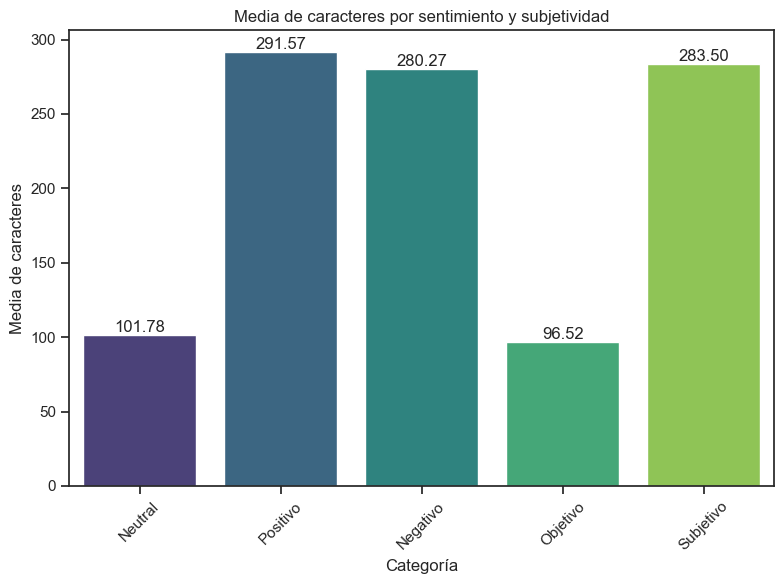
\includegraphics[width=12cm]{Images/Promedio_de_caracteres}
	\caption{Distribución de promedio de caracteres por sentimiento y objetividad.}
	\label{fig:promediodecaracteres}
\end{figure}

A partir de este patrón se infiere una relación entre el tipo de comentario y la extensión de los mismos, observando una mayor expresión de animo y justificación de sentimientos , se observa que los comentarios neutrales y objetivos contienen significativamente una media de menor palabras en comparación con los comentarios positivos, negativos y subjetivos en donde se identifica un conteo alto de palabras, podemos observar esta misma distribución en el conteo de caracteres.\\

\begin{figure}[h!]
	\centering
	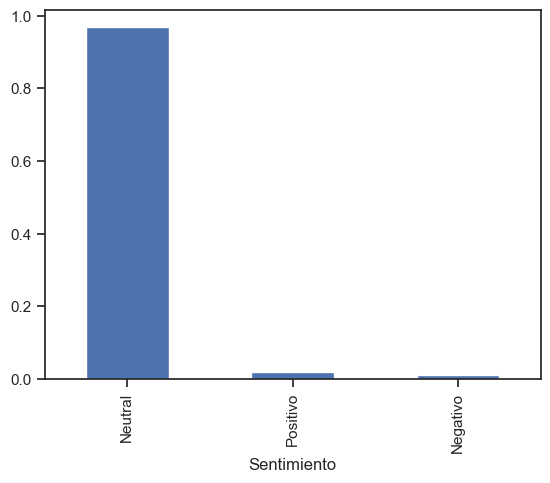
\includegraphics[width=12cm]{Images/Densidad_sentimientos}
	\caption{Distribución de densidad de sentimientos Normalizada.}
	\label{fig:DDSN}
\end{figure}

Al realizar el análisis del de densidad por atributos o clasificación, se identifica una diferencia significativa mayor de comentarios con un sentimiento neutral, a diferencia de aquellos positivos o negativos, estos últimos se presentan un numero significativamente menor, lo que se puede inferir como una respuesta mas concienzuda del publico respecto a sus comentarios en el video del debate, siendo mayor la densidad de comentarios con un sentimiento positivo en comparación con aquellos con una connotación negativa \ref{fig:DDSN}.\\
 
\begin{figure}[h!]
	\centering
	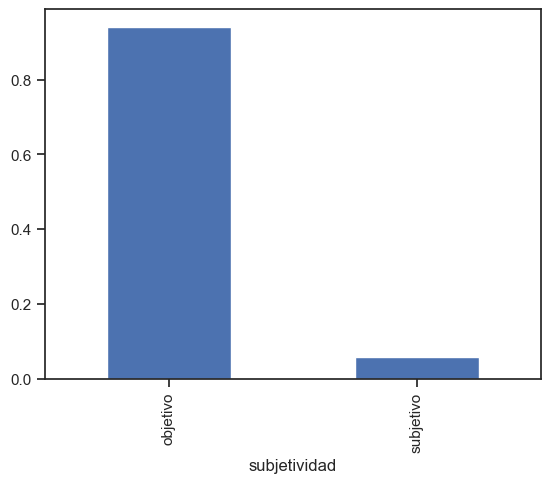
\includegraphics[width=12cm]{Images/Densidad_subjetividad}
	\caption{Distribución de densidad de subjetividad Normalizada.}
	\label{fig:DDSbN}
\end{figure}

Podemos observar en la distribución de densidad en el grafico de subjetividad, una mayor densidad de comentarios de atributo objetivo que aquellos subjetivos, lo que puede indicar que en general el video del debate presenta una tendencia alta de comentarios objetivos que subjetivos.\\

Mientras que al comparar la distribución de las palabras con sentimiento, positivo, neutral, negativo, objetivas y subjetivas, podemos apreciar una alta tendencia a de palabras objetivas y neutrales, sin embargo el resto de atributos presentan 

\begin{figure}[h!]
	\centering
	\includegraphics[width=12cm]{Images/Palabras_sentimiento}
	\caption{Conteo de palabras y su parámetro de sentimiento.}
	\label{fig:CPPS}
\end{figure}

\begin{figure}[h!]
	\centering
	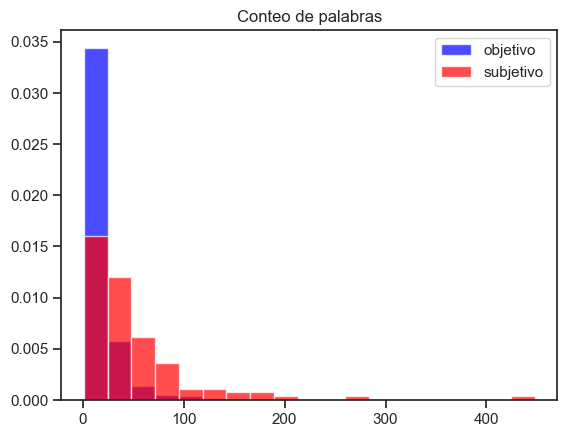
\includegraphics[width=12cm]{Images/Palabras_objetividad}
	\caption{Conteo de palabras y su parámetro de objetividad.}
	\label{fig:CPPo}
\end{figure}
\chapter{Conclusiones}

De manera general se concluye que al realizar una comparación de modelos y atributos, podemos obtener información relevante sobre la tendencia de los sentimientos y objetividad en comentarios 

